\section{Amplificateur opérationnel}
%\vspace{-1\baselineskip}
\textbf{Saturation:} \hspace{1.25cm}\( V_{CC-} < V_o < V_{CC+} \)

\subsection{Ampli-op en mode amplificateur}
En mode amplificateur, on doit analyser le circuit avec deux suppositions importantes:
% %\vspace{-1\baselineskip}
\begin{gather*}
    V_p = V_n\qq{} I_p = I_n = 0
\end{gather*}
%\vspace{-1.5\baselineskip}
\subsubsection{Procédure générale}
La méthode générale à suivre lorsqu’on solutionne des problèmes d’un ampli-op en mode amplificateur est la suivante :
\begin{enumerate}
    \item Calculer la tension à la borne positive, $V_p$. Il ne faut pas oublier que $I_p = 0$
    \item Faire la somme des courants à la borne négative, tout en n’oubliant pas que $I_n = 0$
    \item Appliquer le principe que $V_n = V_p$
    \item Solutionner pour $V_o$ en fonction de $V_i$
    \item Vérifier que $V_{CC-} < V_o < V_{CC+}$
\end{enumerate}

\subsection{Amplificateur inversant}
%\vspace{-1\baselineskip}
\begin{multicols*}{2}
\centering
%  trim={<left> <lower> <right> <upper>}
\includegraphics[trim={2.5in 6.25in 2.5in 3in}, clip=true,page=4,height=1.5in]{fig/fig.pdf}

\begin{equation*}
    V_o = -\frac{R_f}{R_s}V_i
\end{equation*}
\end{multicols*}



\subsection{Amplificateur non-inversant}
%\vspace{-1.5\baselineskip}
\begin{multicols*}{2}
\centering
%  trim={<left> <lower> <right> <upper>}
\includegraphics[trim={2.75in 7.625in 2.75in 1.125in}, clip=true,page=6,height=2in]{fig/fig.pdf}

\begin{equation*}
    V_o = \qty(1+\frac{R_f}{R_s})V_i
\end{equation*}
\end{multicols*}
%\vspace{-1.5\baselineskip}


\subsection{Sommateur}
%\vspace{-1.5\baselineskip}
\begin{multicols*}{2}
\centering
%  trim={<left> <lower> <right> <upper>}
\includegraphics[trim={2.5in 6.75in 2.5in 2.25in}, clip=true, page=5, height=1.5in]{fig/fig.pdf}

\begin{equation*}
    V_o = -R_f\qty(\frac{V_a}{R_a}+\frac{V_b}{R_b}+\frac{V_c}{R_c})
\end{equation*}
\end{multicols*}


\subsection{Amplificateur différentiel}
%\vspace{-1.25\baselineskip}
\begin{multicols*}{2}
\centering
%  trim={<left> <lower> <right> <upper>}
\includegraphics[trim={2.5in 7.625in 2.5in 1.125in}, clip=true,page=7,height=1.5in]{fig/fig.pdf}

\begin{equation*}
    V_o = \frac{R_d}{R_a}\qty(\frac{R_a + R_b}{R_c + R_d})V_b-\frac{R_b}{R_a}V_a
\end{equation*}
\end{multicols*}
\raggedleft
\vspace{-2\baselineskip}
Si \( \frac{R_a}{R_b} = \frac{R_c}{R_d}\) alors, \(V_o = \frac{R_b}{R_a}\qty(V_b-V_a)\)


\subsection{Le comparateur}
%\vspace{-1\baselineskip}
\begin{multicols*}{2}
\centering
%  trim={<left> <lower> <right> <upper>}
\includegraphics[trim={2.5in 8in 2.5in 1in}, clip=true,page=10,height=1.25in]{fig/fig.pdf}

Fonctionnement :
\begin{itemize}[nosep]
    \item \(V_p > V_n\), \(V_o = V_{CC+}\)
    \item \(V_n > V_p\), \(V_o = V_{CC-}\)
\end{itemize}
\end{multicols*}